\documentclass[10pt,a4paper]{article}

\usepackage[utf8]{inputenc}
\usepackage[spanish,provide=*]{babel}
\usepackage[margin=2.5cm]{geometry}
\usepackage{amsmath,amssymb}
\usepackage{graphicx}
\usepackage{booktabs}
\usepackage{hyperref}
\usepackage{microtype}

\title{\vspace{-1cm}\textbf{\LARGE Análisis de Count-Min Sketch y CountSketch en Detección de Ataques mediante Ventanas Deslizantes}\\[3ex]
\large Tarea 1 : Tópicos en Grandes Volúmenes de Datos}

\author{
  \textbf{Joaquín Arriagada Beltrán} \\
  {\small Matrícula: 2022412071} \\[2ex]
  \textbf{Benjamin Díaz Villalobos} \\
  {\small Matrícula: 2022439564} \\[2ex]
  \textbf{Vicente Hernández Guerraty} \\
  {\small Matrícula: 2022412607}
}

\date{\vspace{2ex} 
  Fecha: 1 de octubre de 2026 \\[1ex]
  {{Profesores:} Cecilia Hernández, Álvaro Guzmán}
}
\begin{document}

\maketitle
\vspace{1cm}

\section{Introducción}

El siguiente informe analiza el desempeño de dos estructuras de datos probabilísticas de tipo sketch para la compactación de volúmenes masivos de datos en espacios sublineales: Count-Min Sketch (CMS) y CountSketch (CS). El propósito es comprender y evaluar cómo estas estructuras gestionan el tráfico de datos en redes de alta velocidad bajo restricciones de memoria y tiempo, con el principal objetivo de caracterizar estos parámetros, validar la capacidad de detección de Heavy Hitters junto con su respectiva latencia temporal, y analizar la efectividad de la estimación de cambio de frecuencias entre ventanas consecutivas utilizando vectores firmados.


En este trabajo se implementa un sistema de monitoreo continuo bajo el modelo de ventana deslizante ($W = 60\text{ s}$, con paso $\Delta = 10\text{ s}$), estructurado sobre un anillo circular de 6 subventanas temporales. Gracias a la linealidad, el estado acumulado de la ventana activa se actualiza de manera incremental con costo computacional independiente de la densidad de paquetes. El sistema es sometido a evaluación utilizando trazas reales del proyecto MAWI, sobre las cuales se inyectan dos ataques sintéticos controlados: un ataque de denegación de servicio distribuido (DDoS, monitoreado por IP de destino) y un escaneo masivo de puertos (Scan, monitoreado por IP de origen).

\section{Diseño e Implementación de la Ventana Deslizante}
\subsection{Linealidad y Estructura en Anillo}

Cada sketch mantiene un anillo de $m=6$ sub-sketches $S_q$ y un agregado $A$: siete arreglos de $d\times w$ contadores de 64 bits, esto es, $7\,d\,w\cdot 8$ bytes por tipo de sketch, constantes durante toda la ejecución. Al llegar un paquete se actualizan el sub-sketch vigente y $A$ ($2d$ contadores). Al rotar una subventana se resta su sub-sketch de $A$ ($A\leftarrow A-S_{\text{exp}}$), se limpia y su ranura se reutiliza para la subventana entrante, con un costo de $O(dw)$ independiente de $N_j$. El mismo mecanismo sirve para CMS y CS; solo cambian la actualización (signo $s_r(x)$ en CS) y el estimador (mínimo o mediana).


\subsection{Alineación de Subventanas y Verificación de $N_j$}

La subventana $q$ cubre $(t_0+(q-1)p,\;t_0+qp]$, con $t_0$ el instante del primer paquete, y le corresponde la ranura $(q-1)\bmod m$. Las evaluaciones ocurren en $\tau_j=t_0+W+jp$: en cada una se \emph{expira} primero la subventana más antigua y después se \emph{carga} la nueva, y el anillo se precarga en $\tau_0$ con las seis primeras subventanas. Para $\Delta f$ se calcula $\Delta A_j=S_{\text{entra}}-S_{\text{sale}}$ antes de limpiar la ranura, sin copiar $A_{j-1}$.

Un anillo de seis contadores escalares entrega $N_j$ exacto. Su valor coincidió con la columna $N$ de \texttt{exact\_hh} en las 84 ventanas de cada una de las 8 corridas (traza base por \texttt{src} y \texttt{dst}, y DDoS y Scan con $w\in\{256,1024,4096\}$), lo que valida la alineación.

\section{Actividad 1: Validación y Análisis de Error y Memoria}
\subsection{Metodología de Validación sobre Traza Base}

Se usó la traza MAWI \emph{samplepoint-F} del 3 de diciembre de 2018 (14:00 JST), de unos 900 s y $\approx 123{,}4$ M de paquetes, con $N_j\in[7{,}4;\,8{,}8]$ M y por tanto $T_j=\lceil 0{,}01N_j\rceil\approx 74$--$88$ mil. Se consultaron las cuatro IP más frecuentes por \texttt{src} y por \texttt{dst} (84 ventanas $\times$ 4 claves) con $d=5$ y $w\in\{256,1024,4096\}$, comparando contra \texttt{exact\_hh}. La memoria de contadores es $7\,d\,w\cdot 8$ B: 70 KiB, 280 KiB y 1,09 MiB, idéntica para CMS y CS.

\begin{table}[!htbp]
\centering\small
\caption{Validación en la traza sin ataque: error absoluto medio (MAE, paquetes) y error relativo medio (MRE, \%).}
\label{tab:validacion}
\begin{tabular}{llrrrrr}
\toprule
Clave & $w$ & Memoria & MAE CMS & MRE CMS & MAE CS & MRE CS \\
\midrule
src & 256  & 70 KiB   & 6959,5 & 2,98   & 2613,6 & 1,30 \\
src & 1024 & 280 KiB  & 997,1  & 0,31   & 496,6  & 0,11 \\
src & 4096 & 1,09 MiB & 131,8  & 0,05   & 81,2   & 0,03 \\
dst & 256  & 70 KiB   & 8240,7 & 992,80 & 926,1  & 15,27 \\
dst & 1024 & 280 KiB  & 1517,8 & 162,03 & 214,2  & 8,86 \\
dst & 4096 & 1,09 MiB & 346,2  & 37,43  & 27,0   & 2,12 \\
\bottomrule
\end{tabular}
\end{table}

\subsection{Compromiso Precisión vs.\ Memoria (CMS vs.\ CS)}

La memoria de contadores crece linealmente con el ancho ($7\,d\,w\cdot 8$ B), de 70 KiB a 1,09 MiB, mientras que el error decrece con $w$ en ambos estimadores (tabla~\ref{tab:validacion}). CountSketch domina a Count-Min en todos los anchos y tipos de clave: por ejemplo, para \texttt{src} con $w=256$ el MRE de CS es 1,30\,\% frente al 2,98\,\% de CMS, y a $w=4096$ se reduce a 0,03\,\% frente a 0,05\,\%. La ganancia es decreciente: de $w=256$ a $1024$ el error cae un orden de magnitud, pero de $1024$ a $4096$ la mejora es menor, por lo que $w=1024$ ofrece el mejor equilibrio costo-beneficio.

El MRE de \texttt{dst} es mucho mayor (992\,\% para CMS con $w=256$) porque la tabla promedia sobre claves de frecuencia baja: el error absoluto está acotado por las colisiones, pero el denominador $f_j(x)$ es pequeño, y en CMS el sesgo positivo del operador mínimo hace que esas claves queden muy por sobre su valor real. Sobre las observaciones con $f_j(x)\ge 1000$, la mediana del error relativo en $w=256$ es de $+13$\,\% para CMS, mientras que CS permanece centrada en $\approx 0$; el detalle se analiza en la Sección~\ref{sec:comparacion}. La Figura~\ref{fig:frontera} muestra el compromiso precisión-memoria medido sobre las ventanas de ataque de la Sección~\ref{sec:act2}: en ambos ataques, CS alcanza el error de CMS con menos memoria, y el MRE cae en ambas estructuras al crecer $w$.

\begin{figure}[!htbp]
  \centering
  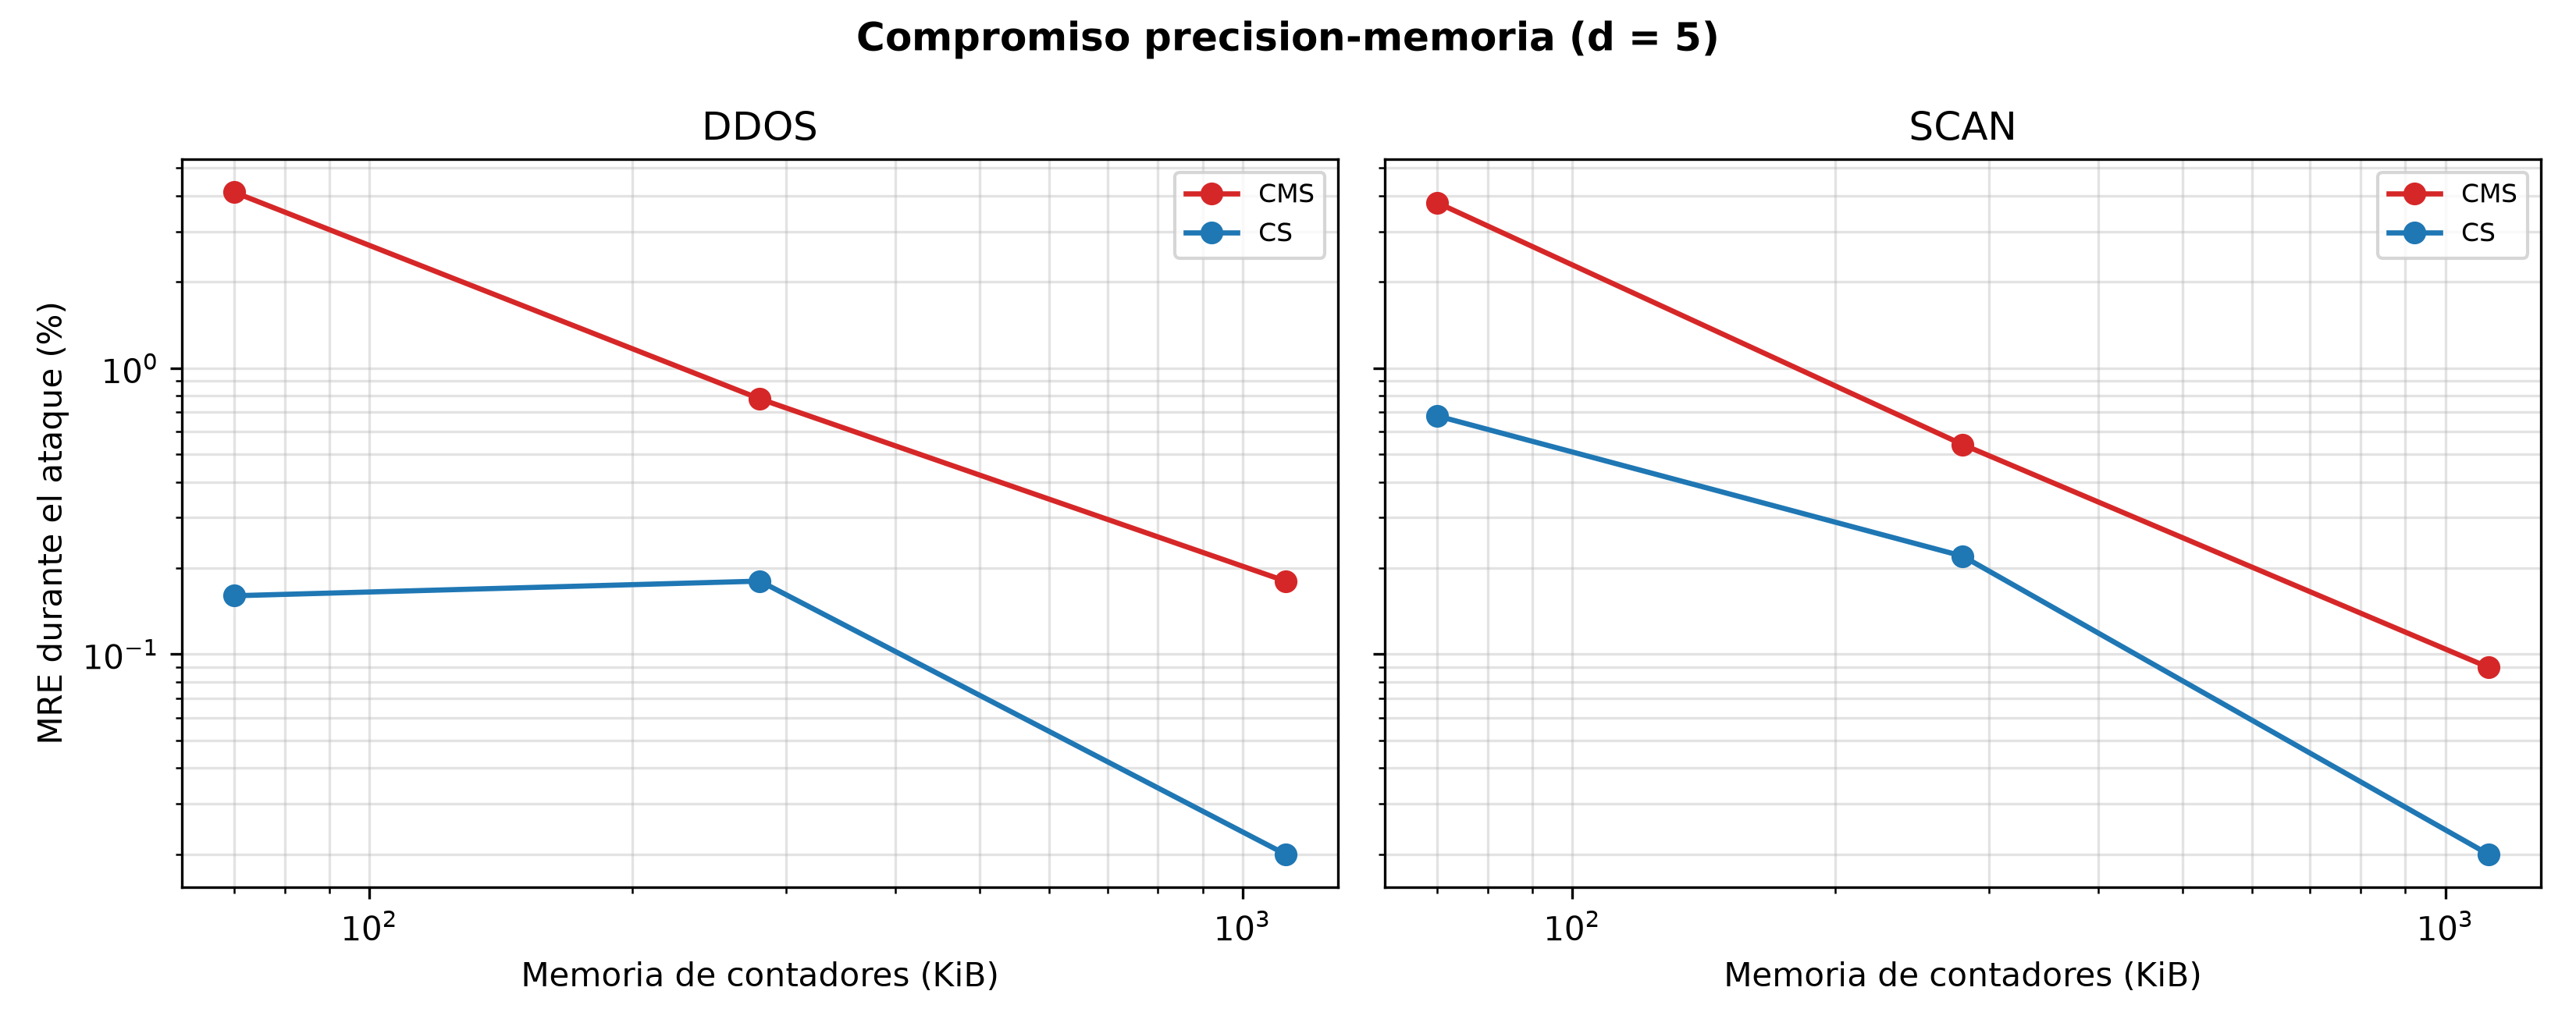
\includegraphics[width=0.7\linewidth]{resultados/figuras/fig_frontera_mre_mem.png}
  \caption{Compromiso precisión-memoria (MRE sobre las ventanas del ataque) para CMS y CS con $w\in\{256,1024,4096\}$, $d=5$. Escalas logarítmicas.}
  \label{fig:frontera}
\end{figure}

\section{Actividad 2: Detección de Ataques DDoS y Scan}\label{sec:act2}

\subsection{Configuración Experimental y Criterio de Heavy Hitters}

Se inyectaron dos ataques sobre la misma traza base con \texttt{inject\_attack.py} (semilla $42$; inicio en $t=300$ s, duración 30 s). \textbf{DDoS:} 10\,000 pps desde 4\,000 fuentes hacia la víctima 163.210.30.13 (destino de ranking 1000 en la traza); se observa la frecuencia por IP de destino. \textbf{Scan:} 8\,000 pps desde 198.18.0.7 hacia 60\,000 destinos; se observa la frecuencia por IP de origen. Un ataque se considera detectado en la primera ventana donde $\hat f_j(x)\ge T_j$, con $\phi=0{,}01$. El conjunto $J$ de ventanas afectadas son las evaluaciones con $t=310,\dots,380$ s ($|J|=8$). La traza es \url{https://mawi.wide.ad.jp/mawi/samplepoint-F/2018/201812031400.pcap.gz}.

\subsection{Detección y Evolución Temporal de Frecuencias}

\begin{figure}[!htbp]
  \centering
  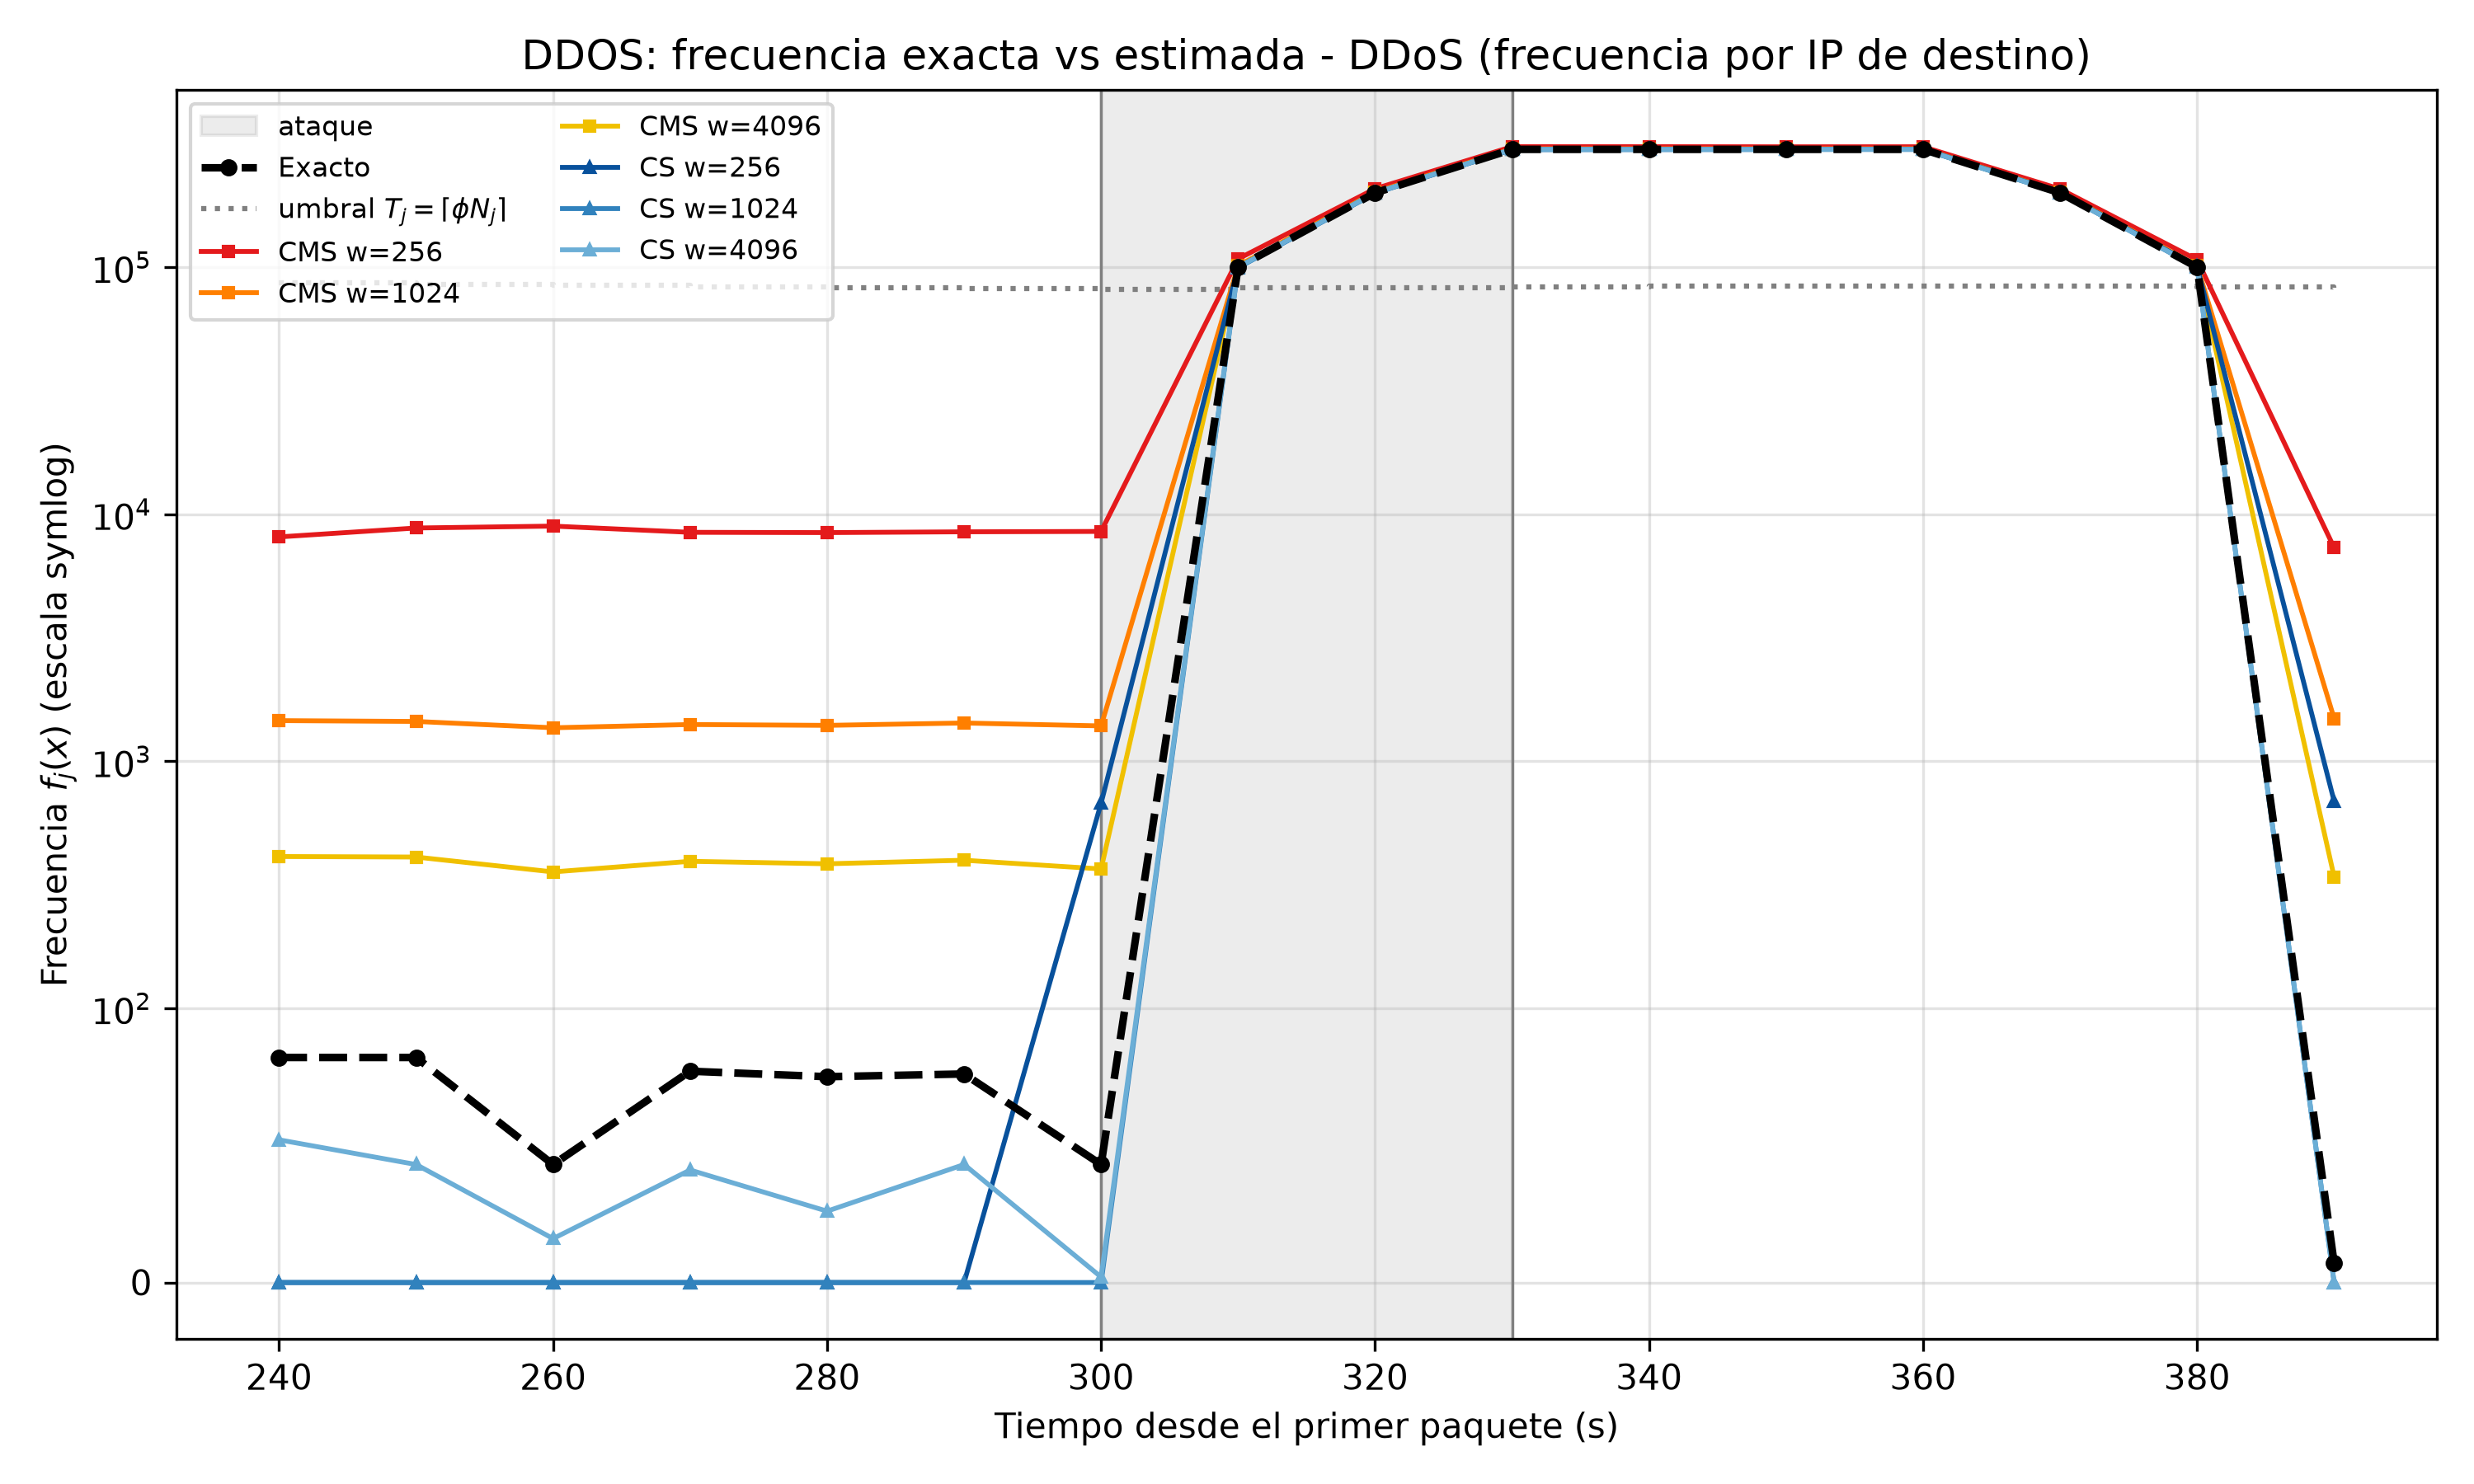
\includegraphics[width=0.49\linewidth]{resultados/figuras/fig_ddos_frecuencia.png}\hfill
  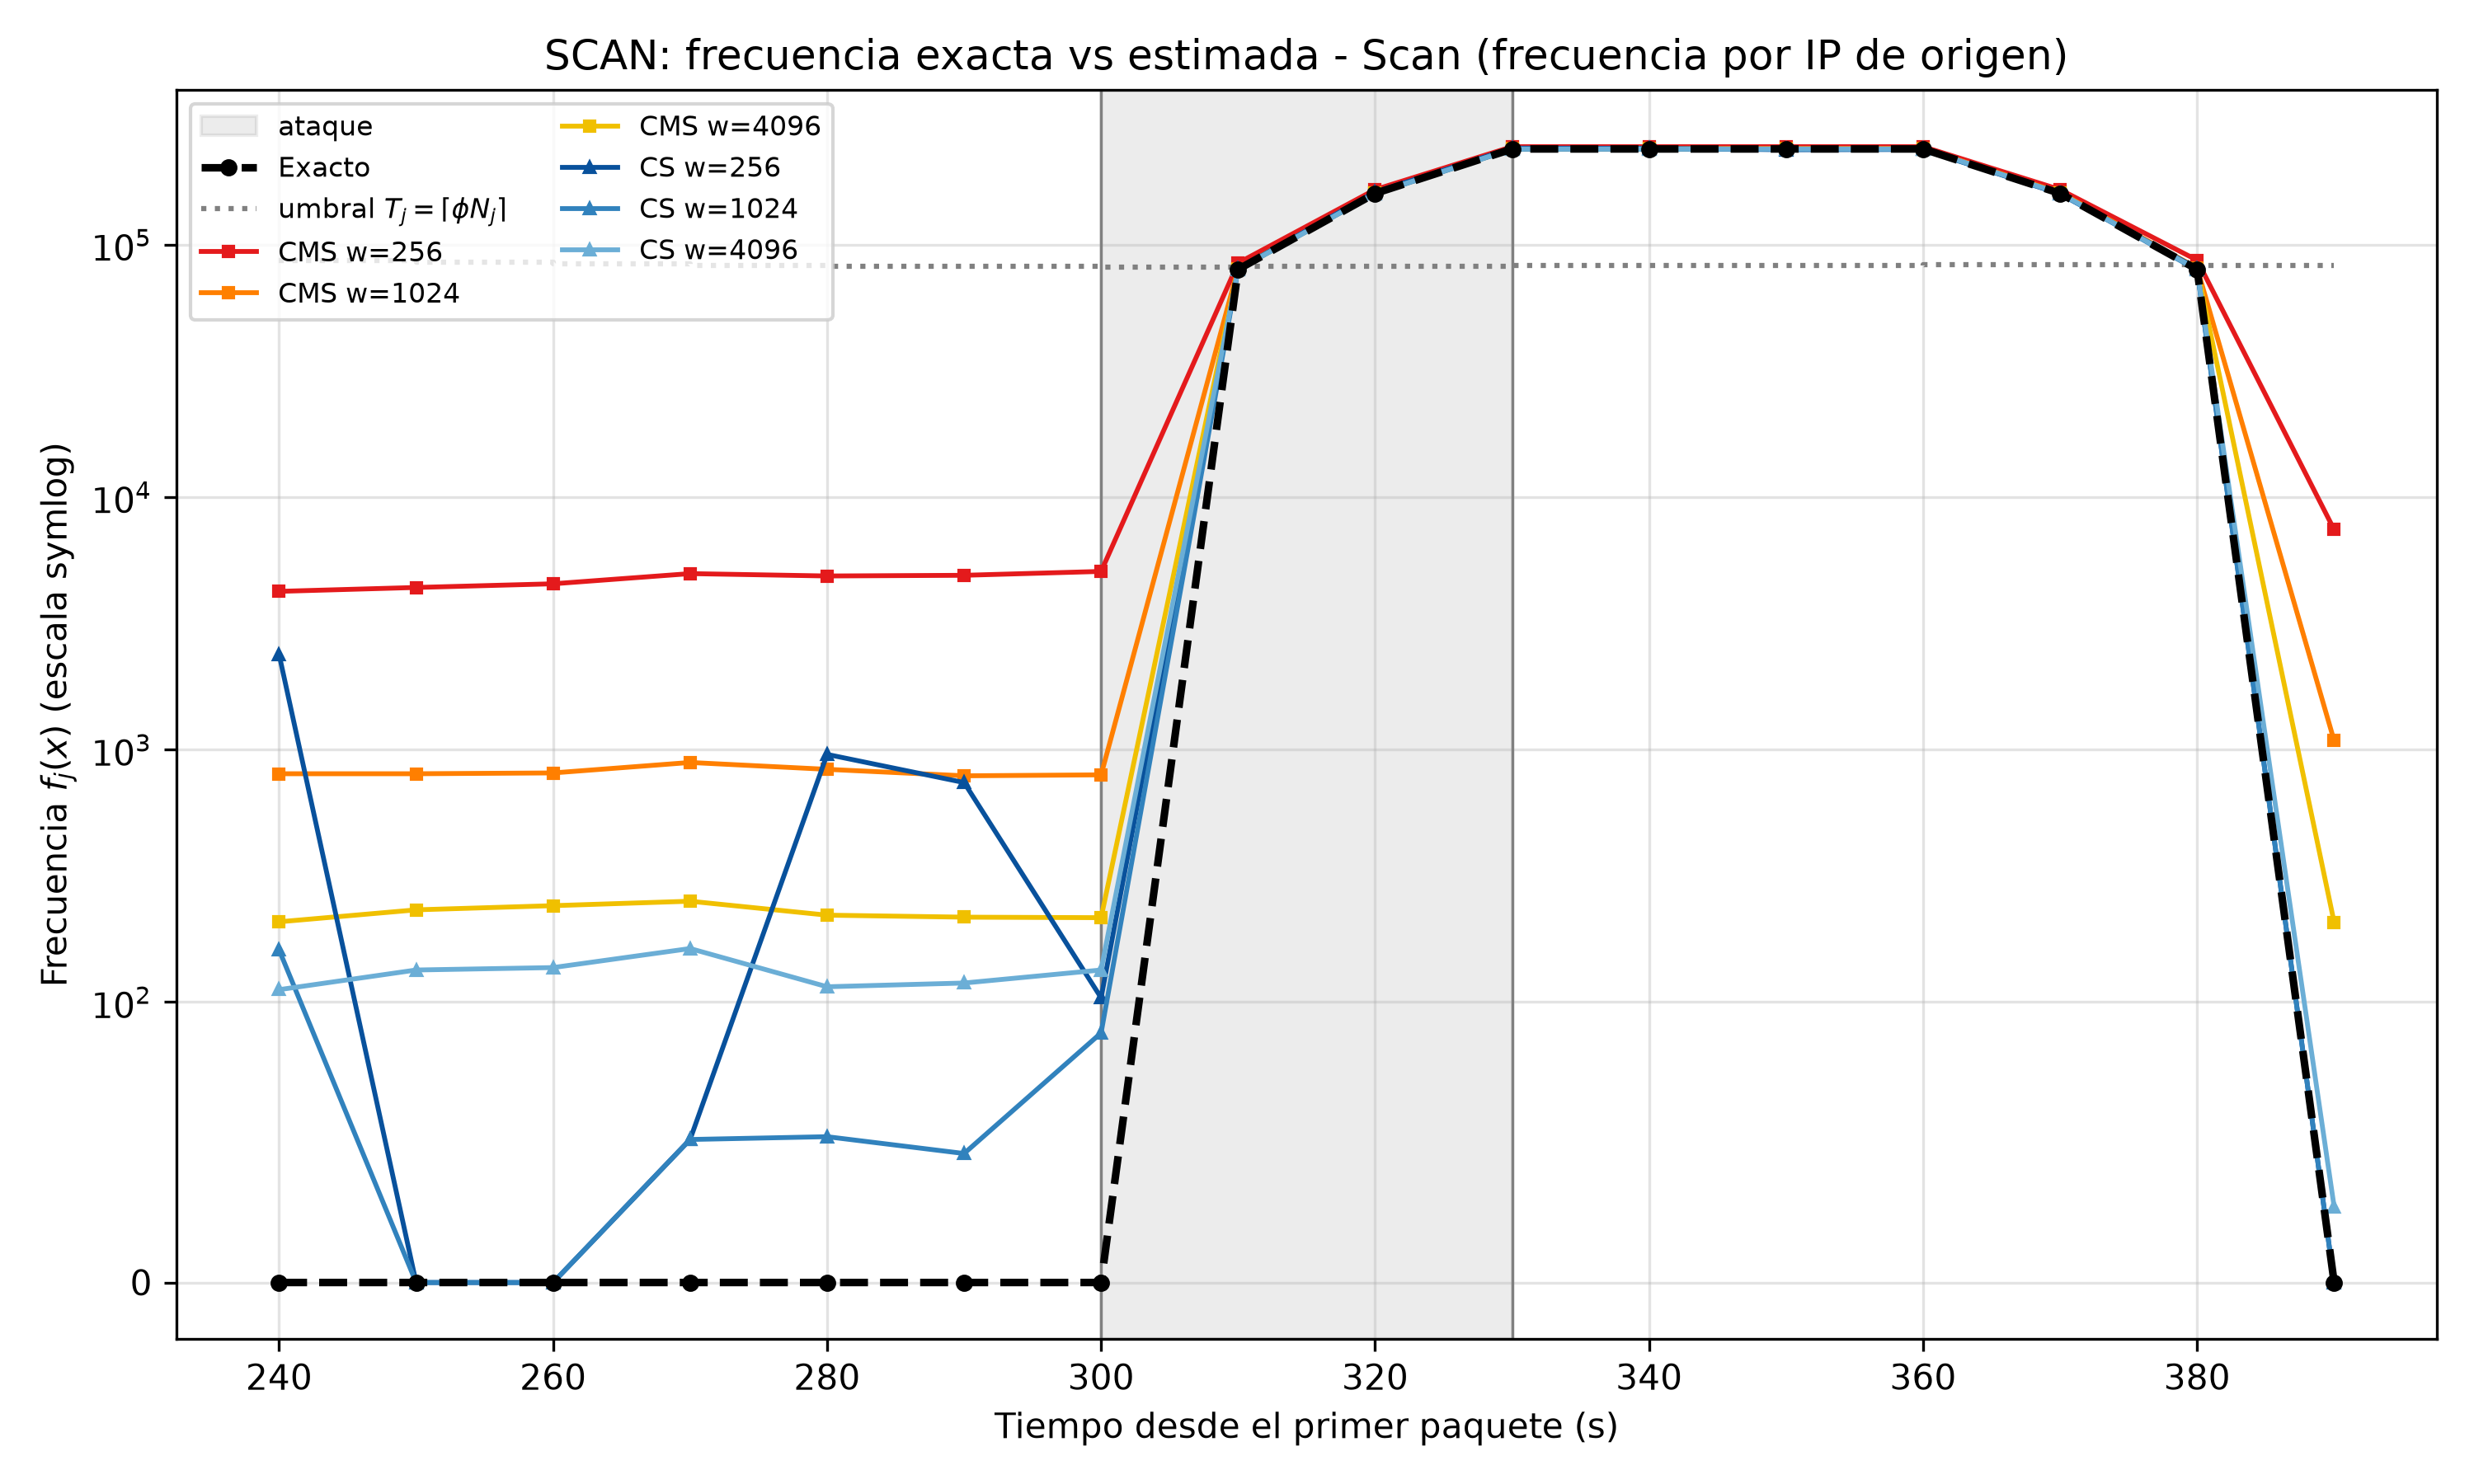
\includegraphics[width=0.49\linewidth]{resultados/figuras/fig_scan_frecuencia.png}
  \caption{Frecuencia exacta y estimada (CMS y CS, $w\in\{256,1024,4096\}$) entre $t=240$ y $390$ s (escala symlog): DDoS por IP de destino (izquierda) y Scan por IP de origen (derecha). La franja gris marca el ataque y la línea punteada el umbral $T_j$.}
  \label{fig:fre}
\end{figure}

\subsection{Análisis de Error Relativo Medio (MRE) y Latencia}

\begin{table}[!htbp]
\centering\small
\caption{Detección: MRE sobre $J$, latencia y falsos positivos (FP). Referencia exacta: latencia de 10 s (DDoS) y 20 s (Scan). FN $=0$ en todos los casos.}
\label{tab:ataques}
\begin{tabular}{llrrrrrr}
\toprule
 & & & \multicolumn{3}{c}{CMS} & \multicolumn{2}{c}{CS} \\
\cmidrule(lr){4-6}\cmidrule(lr){7-8}
Ataque & $w$ & Memoria & MRE (\%) & Lat. (s) & FP & MRE (\%) & Lat. (s) \\
\midrule
DDoS & 256  & 70 KiB   & 4,11 & 10 & 0 & 0,16 & 10 \\
DDoS & 1024 & 280 KiB  & 0,78 & 10 & 0 & 0,18 & 10 \\
DDoS & 4096 & 1,09 MiB & 0,18 & 10 & 0 & 0,02 & 10 \\
Scan & 256  & 70 KiB   & 3,78 & 10 & 2 & 0,68 & 20 \\
Scan & 1024 & 280 KiB  & 0,54 & 20 & 0 & 0,22 & 20 \\
Scan & 4096 & 1,09 MiB & 0,09 & 20 & 0 & 0,02 & 20 \\
\bottomrule
\end{tabular}
\end{table}

\subsection{Comparación CMS vs.\ CountSketch}\label{sec:comparacion}

La Figura~\ref{fig:aprox} contrasta las estimaciones de ambos sketches frente a la frecuencia exacta (19 claves por tipo, 84 ventanas, escala log-log). Count-Min concentra sus puntos por \emph{encima} de la diagonal ($\hat f_j(x)\ge f_j(x)$, sesgo positivo) y el exceso crece con las colisiones ($w$ chico). CountSketch, en cambio, los distribuye simétricamente alrededor de la diagonal: su estimador es insesgado y solo la varianza crece al reducir $w$. La distribución del error relativo (panel derecho) confirma el contraste: la de CMS está corrida a la derecha (mediana $\approx +13$\,\% en $w=256$), mientras que la de CS está centrada en $0$ y se estrecha al crecer $w$.

En la tabla~\ref{tab:ataques} se aprecia la consecuencia práctica: para un mismo $w$, CS entrega menor MRE durante el ataque (0,16\,\% frente a 4,11\,\% en DDoS con $w=256$) con idéntica memoria. En latencia, ambos detectan en la misma ventana que el conteo exacto salvo un caso: \emph{Scan con CMS y $w=256$}, donde CMS declara el ataque una ventana antes que la referencia (latencia de 10\,s frente a 20\,s, con 2 falsos positivos). Esto es el comportamiento esperado del sesgo positivo del mínimo: con $w$ pequeño las colisiones inflan $\hat f_j(x)$ por sobre $T_j$ antes de que la frecuencia real supere el umbral. Es un falso positivo sistemático y previsible, no un error de implementación, y desaparece al crecer $w$ (a $w\ge 1024$ CMS coincide con la referencia). No hubo falsos negativos ($\mathrm{FN}=0$) en ninguna configuración.

\begin{figure}[!htbp]
  \centering
  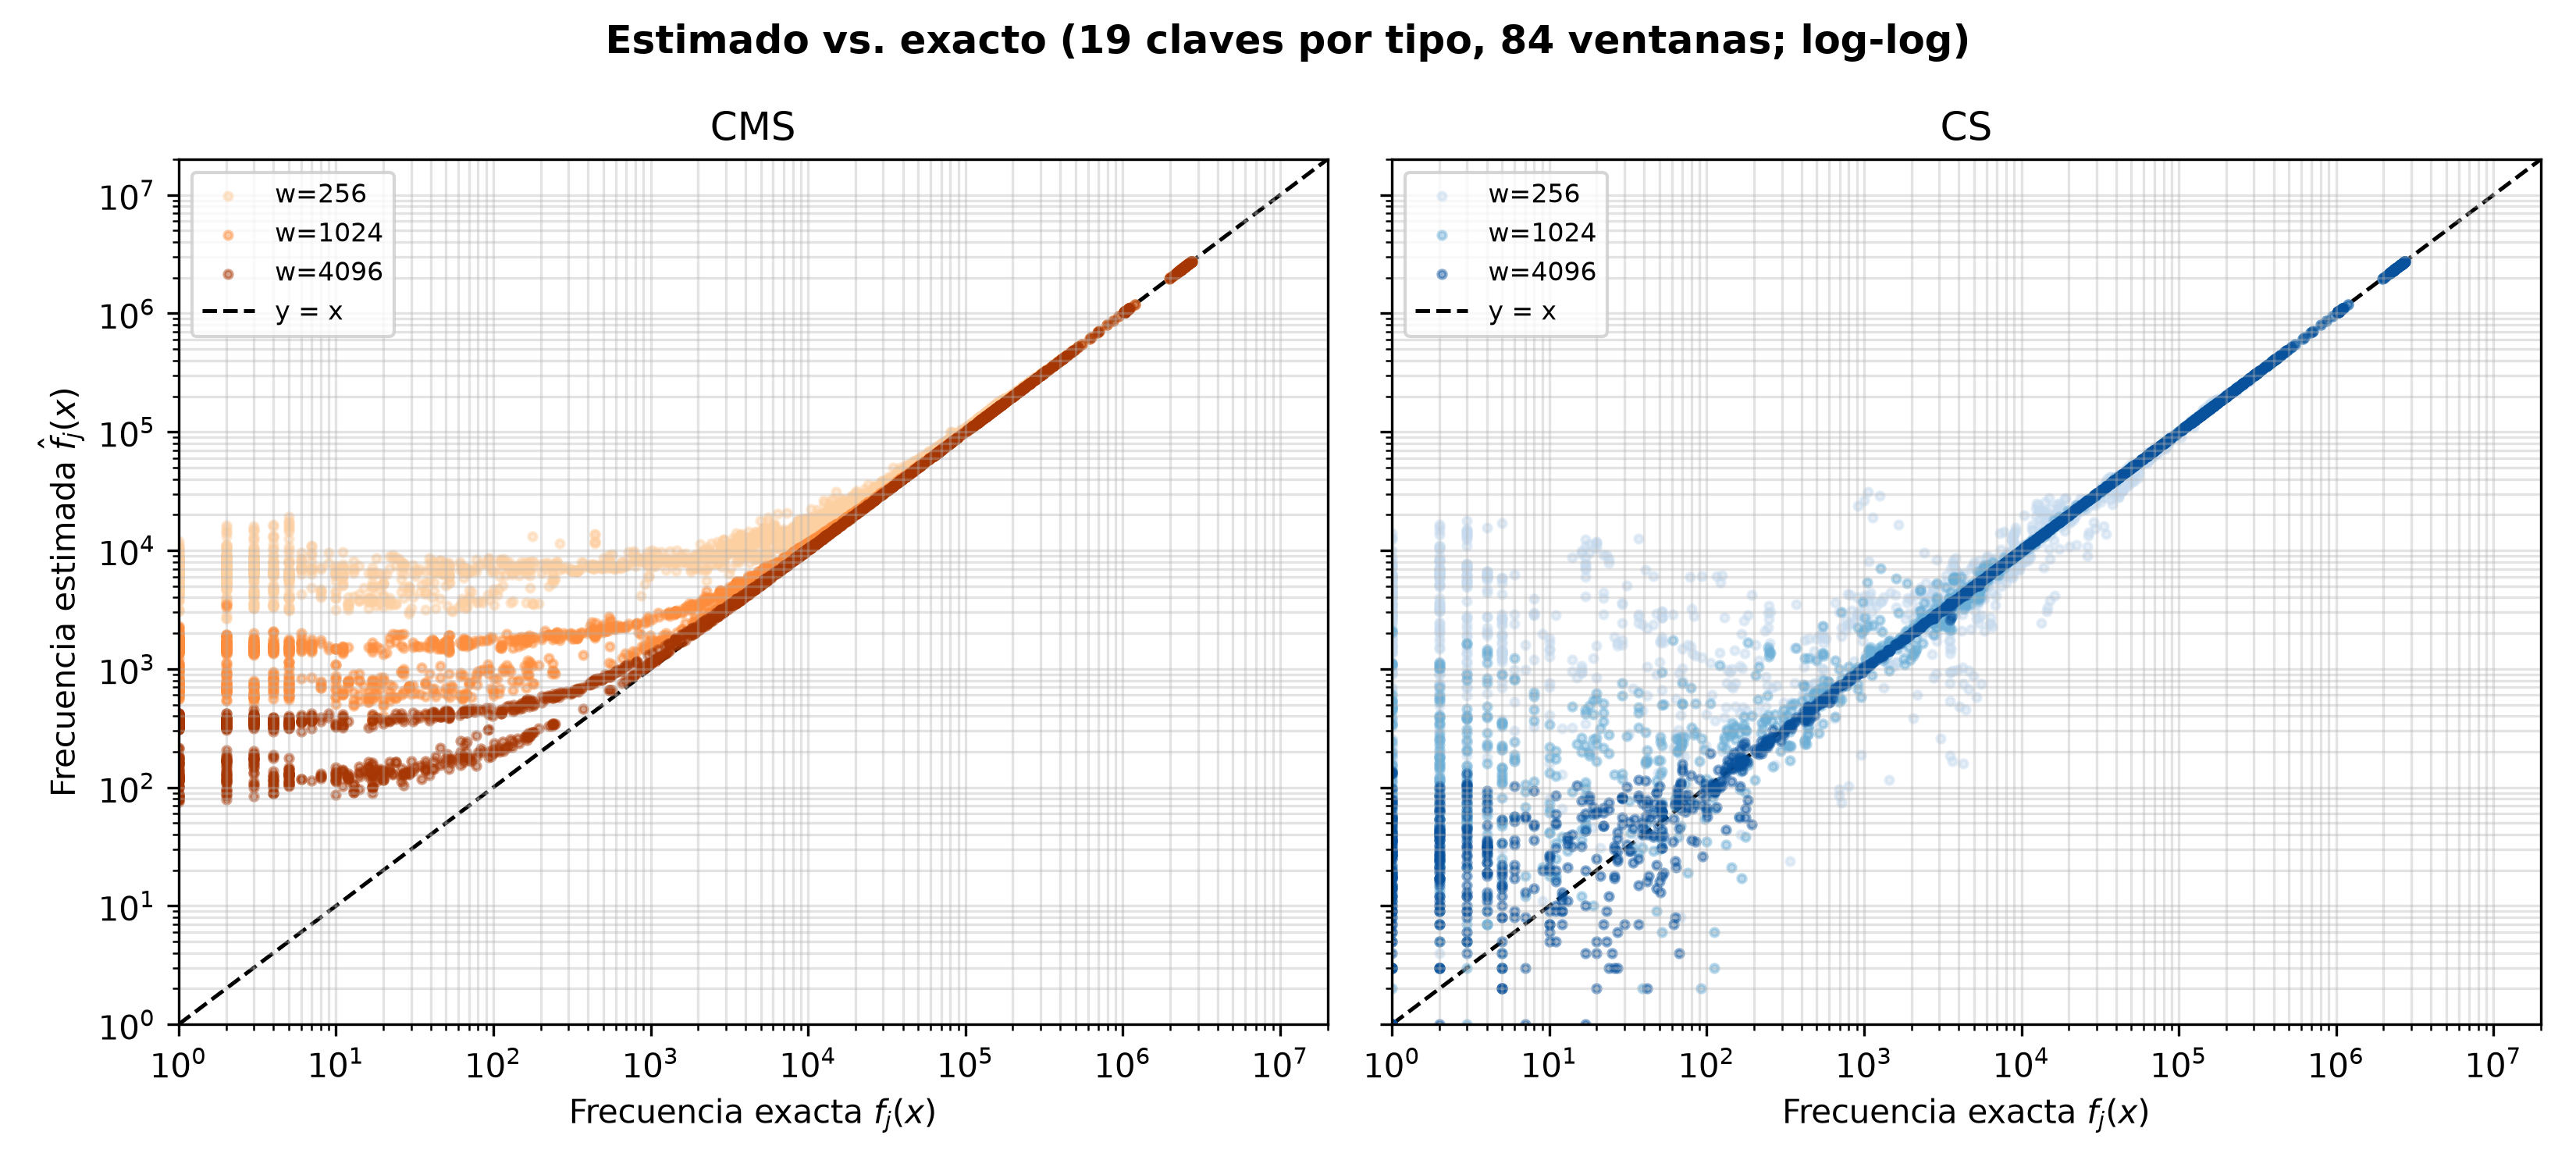
\includegraphics[width=0.55\linewidth]{resultados/figuras/fig_scatter_est_exact.png}\\[2pt]
  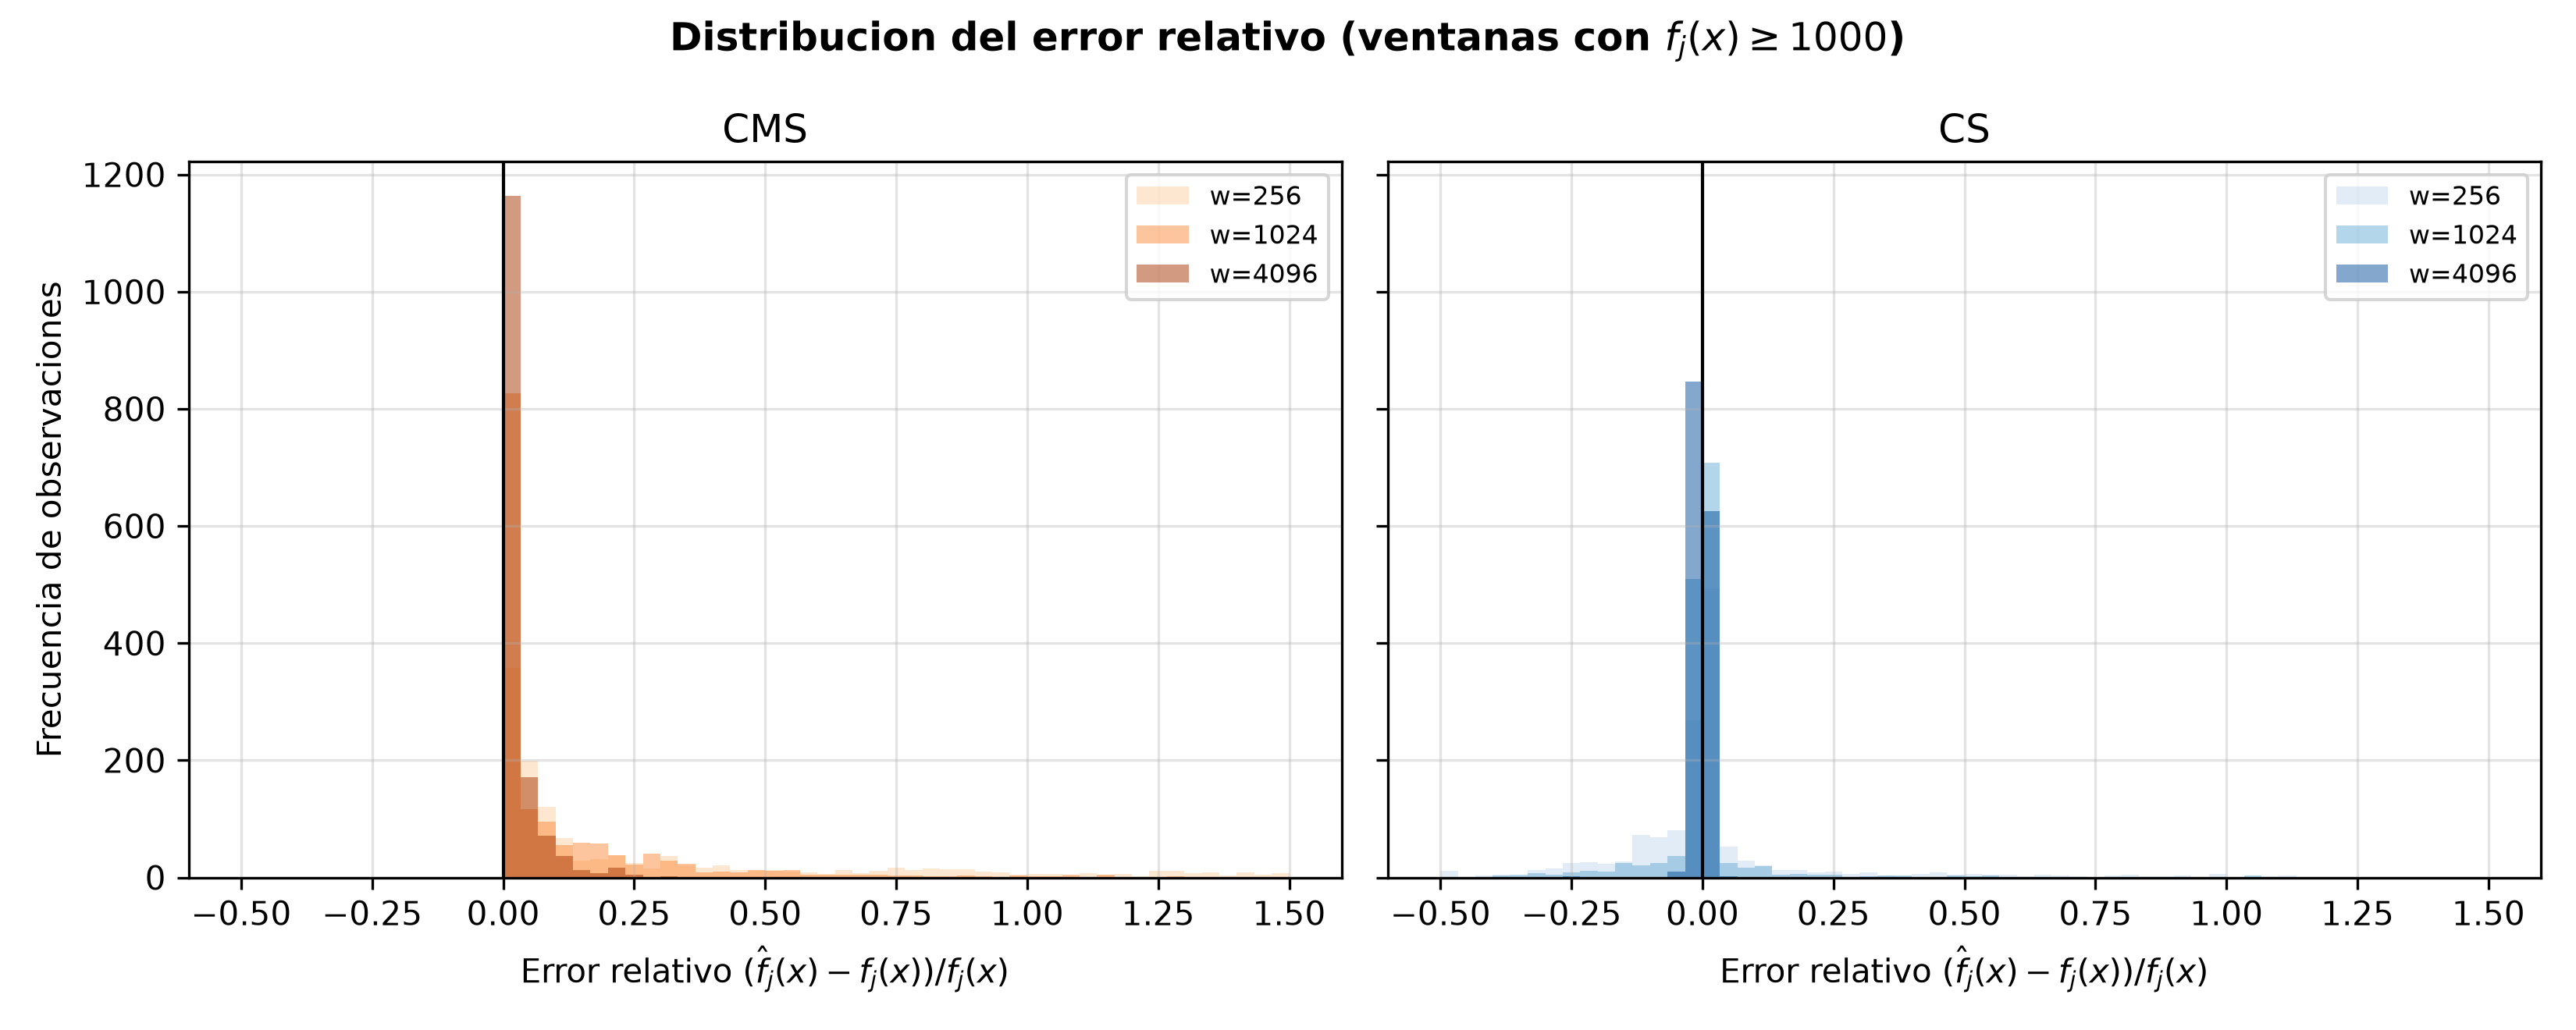
\includegraphics[width=0.55\linewidth]{resultados/figuras/fig_error_hist.png}
  \caption{Estimado vs.\ exacto (arriba, log-log) e histograma del error relativo con $f_j(x)\ge 1000$ (abajo), para CMS y CS con $w\in\{256,1024,4096\}$.}
  \label{fig:aprox}
\end{figure}

\section{Estimación del Cambio de Frecuencia ($\Delta f_j$)}
\subsection{Comportamiento de CountSketch y Variante CMS-Mediana}

\begin{table}[!htbp]
\centering\small
\caption{Error absoluto medio de $\widehat{\Delta f}_j$ en la zona del ataque (9 ventanas, $t=310$--$390$ s).}
\label{tab:delta}
\begin{tabular}{llrr}
\toprule
Ataque & $w$ & CS & CMS-mediana \\
\midrule
DDoS & 256  & 158,8 & 228,6 \\
DDoS & 1024 & 64,8  & 43,7 \\
DDoS & 4096 & 9,1   & 7,6 \\
Scan & 256  & 566,8 & 625,8 \\
Scan & 1024 & 67,1  & 45,0 \\
Scan & 4096 & 16,9  & 12,2 \\
\bottomrule
\end{tabular}
\end{table}

\subsection{Identificación de Picos de Variación e Interpretación}

La Figura~\ref{fig:delta} muestra $\Delta f_j(x)$ exacto junto con las estimaciones de CountSketch y de la variante CMS-mediana. El ataque se manifiesta como un salto positivo abrupto de magnitud igual a la tasa de inyección ($+100\,000$ paquetes por ventana en DDoS y $+80\,000$ en Scan) en $t=310$--$330$ s, y como un decremento simétrico en $t=370$--$390$ s, cuando la subventana que contenía el ataque expira del agregado. Entre ambos, $\Delta f_j\approx 0$: la frecuencia es estacionaria aunque la ventana siga conteniendo todo el ataque, lo que evidencia que $\Delta f$ separa el \emph{cambio} (inicio y fin) del \emph{nivel} (meseta).

En $w=4096$ ambos estimadores recuperan el signo y la magnitud de los picos con error del orden de 1\,\%; a $w\ge 1024$ la variante CMS-mediana resultó ligeramente más precisa en nuestras corridas (tabla~\ref{tab:delta}), mientras que en $w=256$ CountSketch fue más estable. Esto ilustra que, sobre el vector firmado $\Delta A_j$, la mediana captura bien el cambio dominante, pero la ventaja de CountSketch es teórica: sus hashes de signo garantizan insesgadez, mientras que CMS-mediana es una heurística sin cotas cuyo buen resultado en estos datos no está garantizado en general.

\begin{figure}[!htbp]
  \centering
  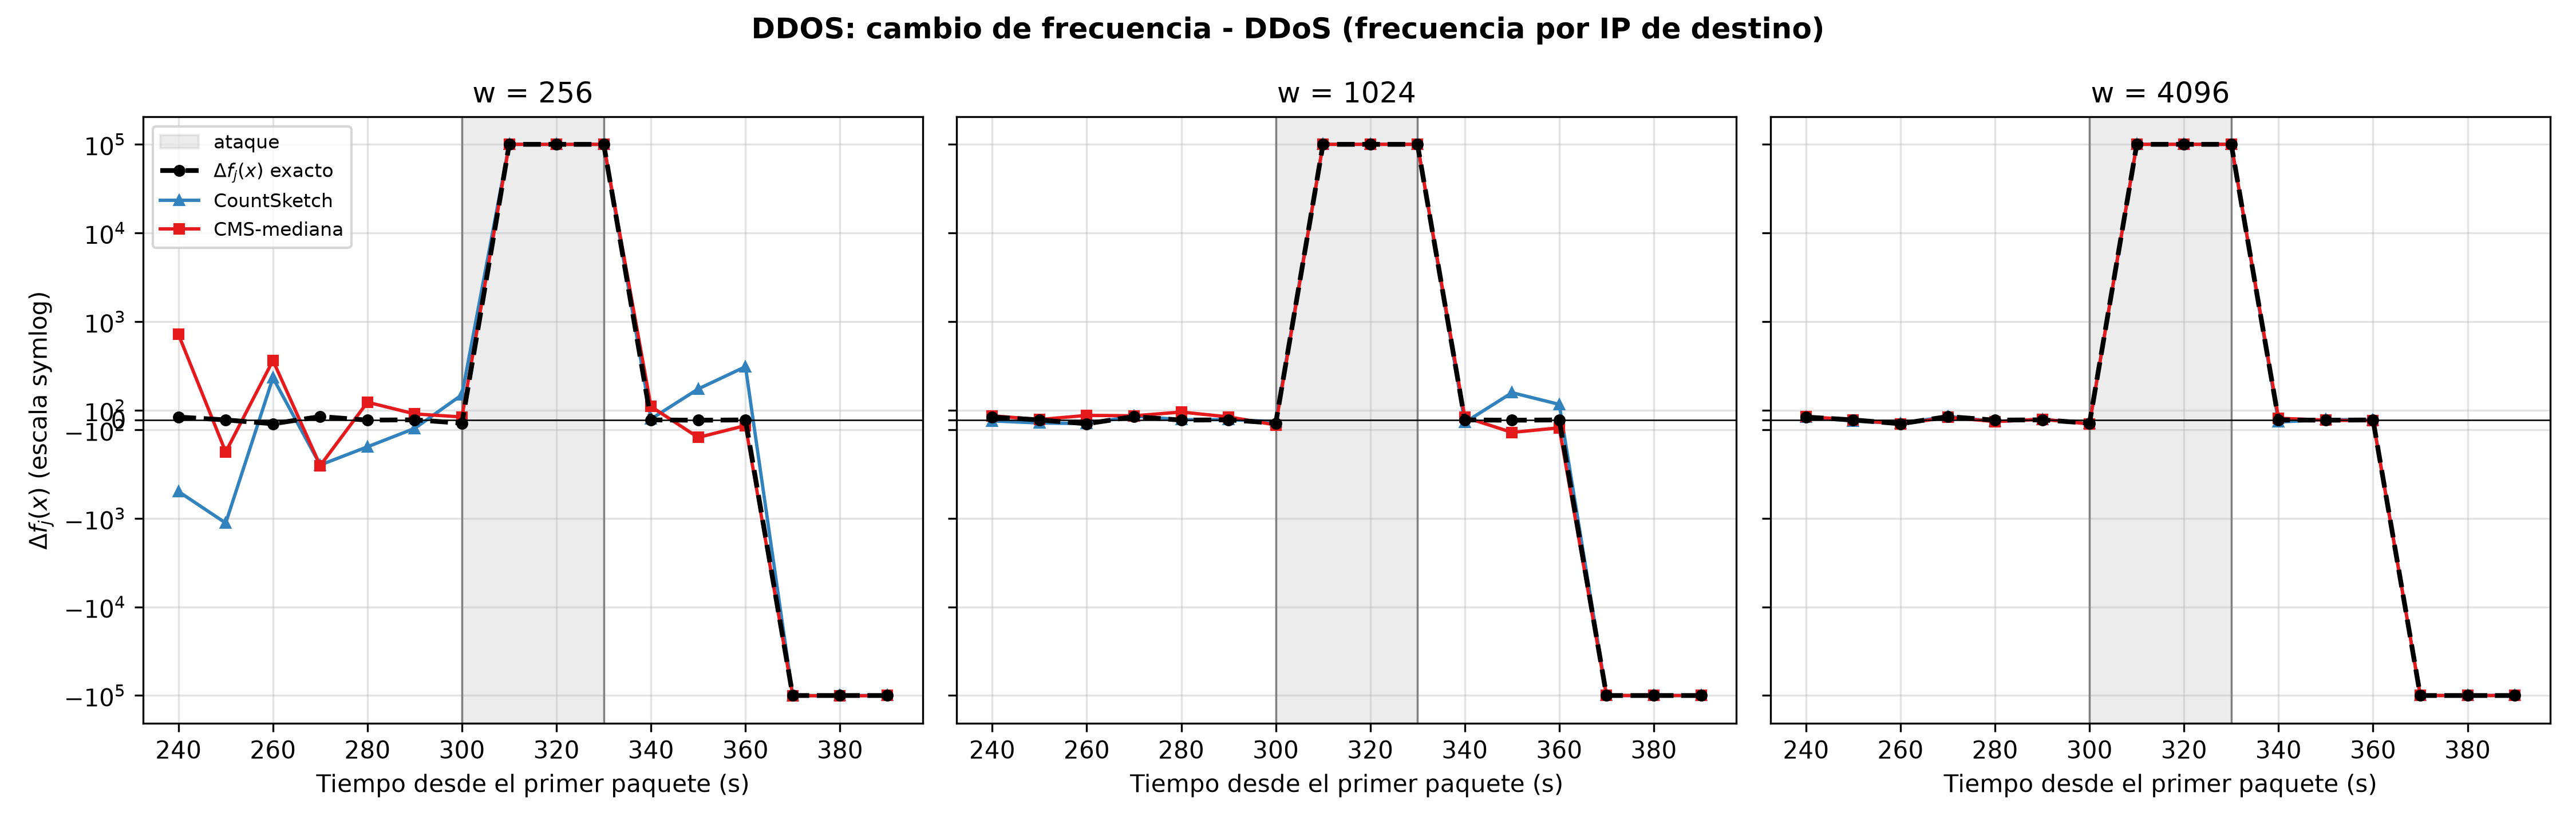
\includegraphics[width=0.55\linewidth]{resultados/figuras/fig_ddos_delta.png}\\[2pt]
  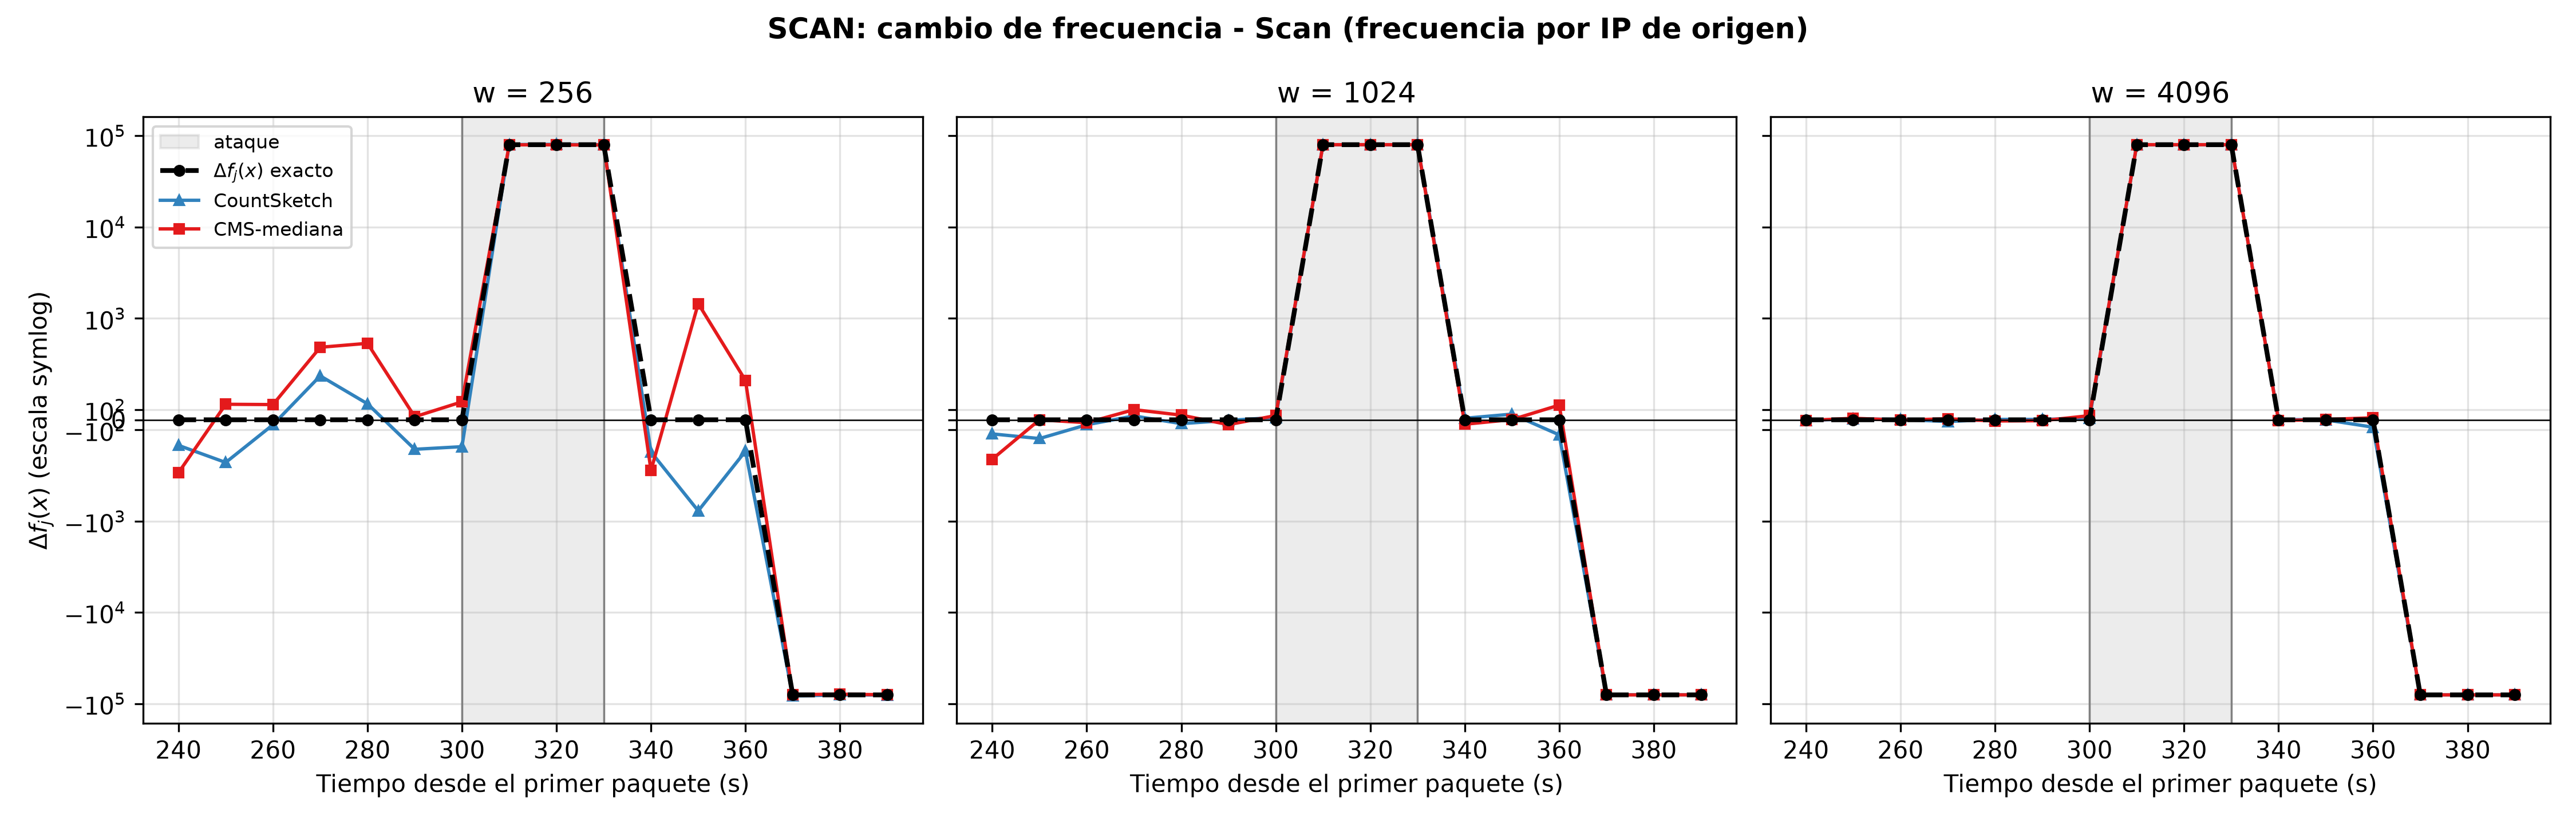
\includegraphics[width=0.55\linewidth]{resultados/figuras/fig_scan_delta.png}
  \caption{Cambio de frecuencia $\Delta f_j(x)$ exacto y estimado (CS y CMS-mediana) para $w\in\{256,1024,4096\}$: DDoS (arriba) y Scan (abajo).}
  \label{fig:delta}
\end{figure}

\section{Preguntas sobre aplicación}

\subsection{¿Por qué la linealidad permite mantener la ventana con costo independiente de la
cantidad de paquetes que permanecen en ella?
}

La linealidad de los sketches garantiza que el resumen de la unión o resta de conjuntos de paquetes equivale a la suma o resta matricial directa de sus celdas ($S_{A \pm B} = S_A \pm S_B$). Gracias a esto, al avanzar de una ventana a la siguiente, no es necesario reprocesar ni reexaminar los paquetes de las $m - 1$ subventanas que continúan vigentes (en nuestro caso, las 5 anteriores al componerse de $m = 6$ subventanas), ya que su información ya se encuentra consolidada en la tabla acumuladora; basta con restar celda a celda el sub-sketch que expira y sumar el que ingresa ($A_{j+1} = A_j - S_{\text{viejo}} + S_{\text{nuevo}}$). De este modo, la actualización depende exclusivamente de las dimensiones fijas de la estructura, con un costo determinista de $O(d \cdot w)$ operaciones elementales, siendo totalmente independiente del volumen de paquetes $N_j$ que permanezca en la ventana activa.

\subsection{¿Qué diferencias observan entre el error de CMS y CS al reducir w?
}
Al reducir el ancho de la tabla $w$, la tasa de colisiones se incrementa en razón de $O(1/w)$, pero sus efectos difieren por cada estructura. En Count-Min Sketch, al registrarse únicamente incrementos positivos y aplicar el operador mínimo, cada colisión añade ruido de forma unilateral, generando un sesgo positivo que crece de forma marcada al reducir $w$ (MRE de 992,80\,\% con $w=256$ en destinos). Por el contrario, CountSketch asocia a cada clave un signo aleatorio $s(x) \in \{-1, +1\}$, lo que hace que las colisiones se cancelen mutuamente al tener una esperanza de ruido nula; de este modo, aunque reducir $w$ incrementa la varianza, el estimador se mantiene insesgado y el operador mediana filtra los valores atípicos, degradando el rendimiento de manera mucho más suave y controlada (en la misma configuración el MRE es de solo 15,27\,\%).

\subsection{¿Cuál de los dos ataques se detecta con mayor claridad y por qué la definición de la
clave es distinta para DDoS y Scan?}

La definición de la clave varía según la convergencia del volumen masivo de paquetes. En DDoS el ataque es producido hacia un único servidor mediante muchas máquinas atacantes, por lo tanto, la clave se ubica en la IP de destino, que es donde se acumulan los paquetes inyectados por segundo. Si fuera en la IP de origen, cada máquina enviaría un flujo diminuto. En cambio en Scan, un único atacante sondea decenas de miles de servidores o puertos distintos, por lo tanto la clave conviene ubicarla en la IP de origen, que es la que emite los miles de paquetes por segundo. Si fuera en la IP de destino solo llegarían unos pocos paquetes.



El ataque detectado con mayor claridad fue Scan. Esto sucede debido al alto contraste que genera frente al tráfico base que existe (en este caso la red habitual MAWI). Estas redes presentan un tráfico moderado y distribuido entre muchos clientes normales, por lo que si el atacante empieza a emitir 8\,000 paquetes por segundo desde una única IP, pasa de casi nulo a un flujo masivo provocando un gran contraste. Esto no sucede en DDoS, que aunque genere mayor volumen absoluto, los servidores de destino de forma natural concentran mucho tráfico legítimo. Aunque la víctima sobrepase el umbral $\phi N_j$, compite con otros destinos activos de la traza, por lo que la relación de señal a ruido respecto a otros flujos grandes es ligeramente más limpia en el Scan por IP de origen.

\subsection{¿Qué información adicional entrega $\Delta f_j(x) = f_j(x) - f_{j-1}(x)$ respecto de observar sólo
la frecuencia de la ventana actual?}

Observar la frecuencia de ventana actual $f_j(x)$ solo refleja el volumen acumulado de paquetes, sin poder diferenciar entre un flujo legítimo de alto tráfico y un ataque. La diferencia de ventanas aporta la velocidad del cambio del flujo, siendo clave para detectar con exactitud el instante de inicio de una anomalía mediante un salto positivo abrupto ($\Delta f_j \gg 0$) en los últimos $\Delta = 10\text{ s}$. Además permite caracterizar el ciclo de vida completo del evento al distinguir su fase activa de régimen estacionario ($\Delta f_j \approx 0$) y su finalización mediante una caída abrupta o un valor fuertemente negativo ($\Delta f_j \ll 0$) originado cuando la subventana que contenía el ataque sale del acumulador.


\subsection{
Compare $\Delta \widehat{f}_j^{\text{CS}}(x)$ y $\Delta \widehat{f}_j^{\text{CMS-med}}(x)$. ¿Por qué CountSketch puede utilizar su estimador habitual, mientras que en CMS se reemplaza el mínimo por una mediana y se pierden las garantías estándar?}

La matriz de diferencias entre ventanas $D_j = A_j - A_{j-1}$ pertenece al modelo con signo: sus celdas pueden ser positivas o negativas según los flujos crezcan o expiren. CountSketch puede usar su estimador habitual de forma directa porque incorpora por diseño hashes de signo $s(x) \in \{-1, +1\}$, lo que garantiza que las colisiones en $D_j$ tengan esperanza nula y que el estimador conserve su insesgadez. En cambio, el estimador clásico de CMS se fundamenta en incrementos estrictamente positivos: aplicar el operador mínimo sobre $D_j$ haría que una colisión con un flujo que decreció drásticamente seleccione el valor más negativo, subestimando arbitrariamente. Para evitarlo, CMS recurre heurísticamente a la mediana, pero al carecer de la propiedad de no-negatividad y del hash de signo que sustentan la desigualdad de Markov, se pierden las cotas teóricas estándar de sobreestimación ($\hat f \ge f$).

\section{Conclusiones}

Se implementaron Count-Min Sketch y CountSketch sobre una ventana deslizante de 60\,s explotando la linealidad: un anillo de 6 sub-sketchs y un agregado $A$ que se actualiza restando la subventana que expira y sumando la entrante, con costo $O(dw)$ independiente de $N_j$. La alineación se validó ventana por ventana contra \texttt{exact\_hh} (84/84 ventanas idénticas en las 8 corridas), lo que garantiza que las diferencias observadas provienen del estimador y no del mecanismo de ventana.

En precisión, CountSketch supera sistemáticamente a Count-Min con la misma memoria: es insesgado (el hash de signo hace que las colisiones se cancelen) y el operador mediana filtra valores atípicos, mientras que CMS acumula un sesgo positivo que crece al reducir $w$ (el mínimo sobreestima). La memoria crece linealmente con $w$ ($7\,d\,w\cdot 8$ B) y $w=1024$ ofrece el mejor equilibrio costo-beneficio.

Ambos sketches detectan DDoS y Scan en la misma ventana que la referencia exacta (latencia de 10--20\,s), salvo el caso esperado de Scan con CMS y $w=256$, que adelanta la detección una ventana por el sesgo del mínimo (falso positivo reportado y explicado). Para el cambio de frecuencia, el vector firmado $\Delta A_j = A_j - A_{j-1}$ permite estimar $\Delta f_j$ sin reprocesar paquetes: CountSketch conserva sus garantías con su estimador habitual, y la variante CMS-mediana —experimental y sin cotas— resultó comparable en la práctica.

En conjunto, para detección en tiempo real sobre tráfico de alta velocidad, CountSketch es la opción más robusta a $w$ pequeño; Count-Min sigue siendo competitivo a $w$ grande, donde su sesgo se vuelve despreciable.

\end{document}